\section{Resultat}
\label{sec:Lieth_Wahid-results}
I detta avsnitt presenteras resultaten som har fåtts från datainsamlingen.
\subsection{Scrum-utvärdering under sprintutvärdering}
Frågor som ställdes i utvärderingen av Scrum ~\ref{Lieth:scrumU} lade stor fokus på de två viktiga aspekterna av Scrum som nämndes tidigare under ~\ref{two} vilka är transparens och granskning.
Transparens är en mycket viktig del av Scrum och därför togs det hänsyn till. Alla medlemmar i teamet var överens om att Scrum-bräde som kom i form av ett Trello-Board gjorde det lättare att veta vilka 
utvecklingsuppgifter tilldelades vilka av teammedlemmarna. Vidare kände teamet sig nöjt med resultaten av i stort sett varje sprint. Svaren på ~\ref{f3} varierade mellan olika sprinter. Till exempel i början av sprint 2 var väldigt få teammedlemmar vana vid Javascript, React och alla essentiella utvecklingsverktygen som behövdes för att utföra projektet. Detta ledde till att tidsestimering var inte riktig korret det vill säga att teamet underskattade vissa delar och överskattade andra delar. Teamet bestämde sig redan från
början att hålla öppenhet och transparens det vill säga att om någon i teamet kände sig osäker på att han kunde klara en uppgift så skulle teamet hjälpa honom. All kodning som skrevs skickades till Github och där granskades den av det automatiserat testningsverktyget Travis men också av en av våra teammedlemmar.

\subsection{Frågeformulär}
Målet med frågeformuläret var att få en klar bild för vad teamet har fått för erfarenheter från att jobba agilt med Scrum, och vilka delar som är essentiella som behöver vara med för ett framgångsrikt studentprojekt. Först och främst behöver man veta om teamet har kunskap inom Scrum teori därför ställdes frågan \textit{Hade du erfarenheter inom Scrum sedan tidigare? } Resultat av svaren på denna fråga visade att mer hälften av teamet inte hade några erfarenheter av att använda Scrum medan resten inte kände sig bekväma med att använda ramverket. Detta innebär att kunskapen inom Scrum utvecklades under projektets gång. Eftersom projektet hade en begränsad tidsbudget på 400 timmar per person lades majoriteten av tiden på utvecklingen samt dokumentskrivningen vilket ledde till att mindre fokus lades på Scrum.  

Utöver det tyckte 71\% av teamet att Scrum har bidragit att hjälpa oss att jobba effektivt. Detta visar att teammedlemmarna är nöjda med valet av utvecklingsmetodiken vilket visar att Scrum mötte vårt behov. Å andra sidan varierade svaren när det kom till att beskriva sina upplevelser av att jobba agilt med Scrum. Mer än hälften av teamet beskrev det som positivt trots svårigheter som teamet har haft för att anpassa sig till Scrum vid början av projektet. Resten av svaren var en blandning av att sprinten var allt för korta eller att Scrum inte har hjälpt speciellt mycket. Anledning till detta blir klarare när man kollar på nästa fråga som handlar om vilka delar av Scrum som saknades. De flesta tyckte att delar som \textit{stå-upp möten} hade  hjälpt teamet att jobba effektivt. Vidare tyckte teamet inte att Scrum var nödvändig för projektets framgång dels för att den inte följdes bra av teamet och dels på grund av vi använde väldigt små delar av Scrum till exempel Scrum-bräde.
Läsaren hänvisas till appendix ~\ref{Leypendix} för att se resten av resultaten av enkäten.

\subsection{Vattenfallsmodellen}
För att kunna jämföra resultaten som ficks från undersökningen av användning av ramverket Scrum mot vattenfallsmodellen valdes en hel del vetenskapliga artiklar. De valda artiklarna är en hel del fallstudier som har genomförts hos olika lärosäten och dokumenterats. Anledning till att dem artiklarna valdes är på grund av att var och en av dem dokumenterar tidigare resultaten som av att använda vattenfallsmodellen och jämför det med resultaten av att använda ramverket Scrum. Det vill säga att artiklarnas fokusområden är relevant för fokusområdet av denna undersökning. Dessutom är artiklarna dokumenterade av professorer och forskare i de respektive lärosäten vilket gör dem mer trovärda. Till exempel artikel \cite{Usingscr27:online} dokumenterar att den projektbaserad kursen som ges vid lärosätet har tidigare konfrontraterats med problemet att kursstudenterna antingen inte kunde leverera ett fullt fungerande projekt eller det levererat projektet var av dålig kvalitet. Projektkursen använde sig då av vattenfallsmodellen. Artikel \cite{GameDesign} dokumenterar liknande resultat vid ett annat lärosäte och menar att anledning till det är på grund av användning av vattenfallsmodellen. Båda artiklarna dokumenterar att användning av ramverket Scrum har varit speciellt givande och lett till att en stor framgång. Dessutom dokumenterar dem att användning av Scrum har lett till en stor förbättring jämfört med tidigare år då alla studenter har kunnat leverera ett fullt fungerande projekt vid slutet av kursen och därmed har uppnått kursmålen.
\\
\begin{figure*}[h]
	\centering
	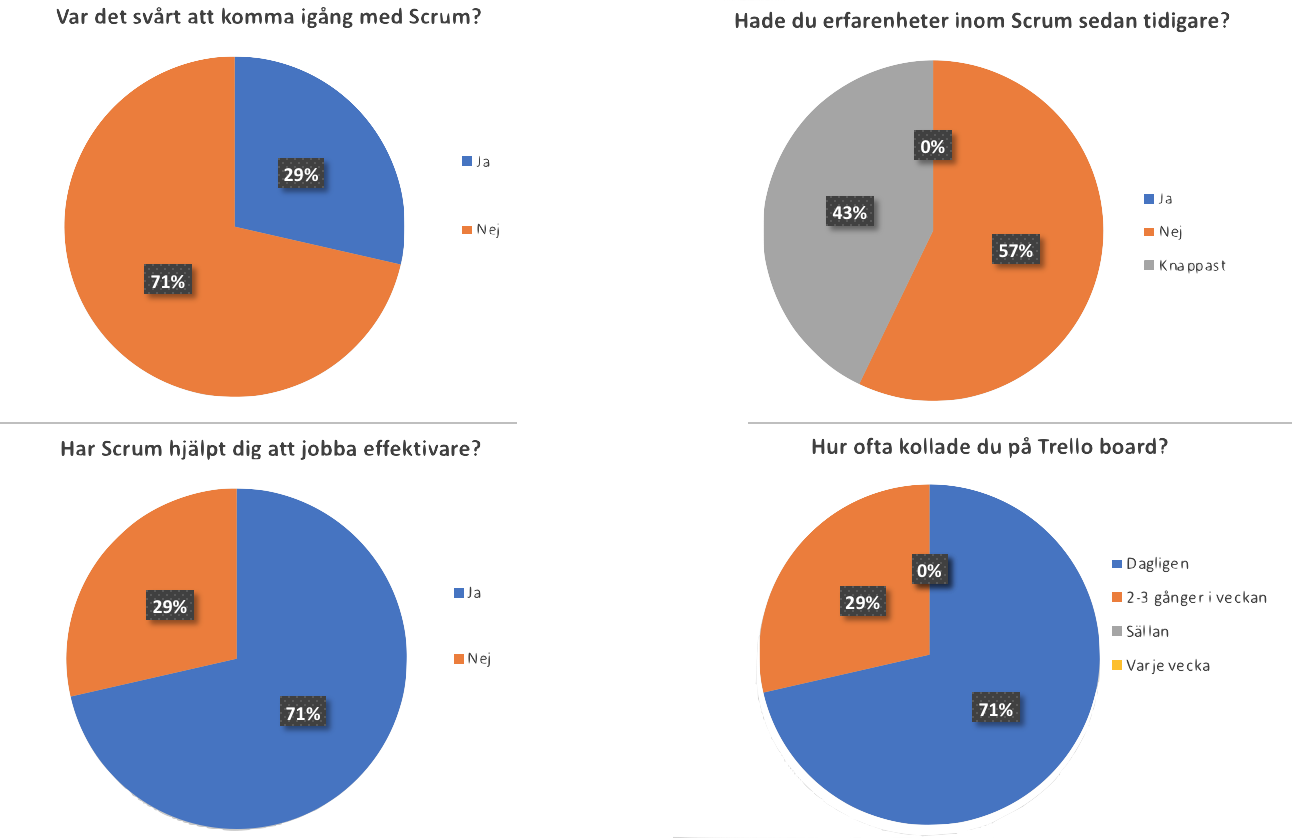
\includegraphics[scale=0.6]{q1_4}
	\caption{Resultat från frågeformuläret}\label{fig1}
	\label{q1}
\end{figure*}
\newpage